\chapter{全域木 - Spanning trees}

\index{spanning tree}

\key{全域木(spanning tree)}は任意の2つのノード間にパスが存在するようなエッジで構成されている木です。
一般的な木と同様、木は連結していてサイクルは存在しません。
木を構成するにはいくつかの方法があります。

次のようなグラフを考えてみましょう。
\begin{center}
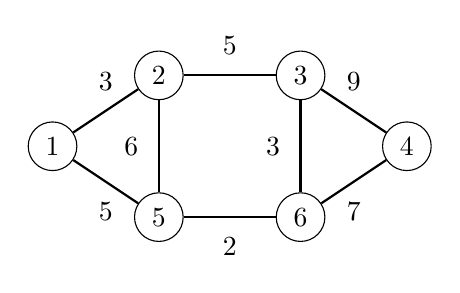
\begin{tikzpicture}[scale=0.9]
\node[draw, circle] (1) at (1.5,2) {$1$};
\node[draw, circle] (2) at (3,3) {$2$};
\node[draw, circle] (3) at (5,3) {$3$};
\node[draw, circle] (4) at (6.5,2) {$4$};
\node[draw, circle] (5) at (3,1) {$5$};
\node[draw, circle] (6) at (5,1) {$6$};
\path[draw,thick,-] (1) -- node[font=\small,label=above:3] {} (2);
\path[draw,thick,-] (2) -- node[font=\small,label=above:5] {} (3);
\path[draw,thick,-] (3) -- node[font=\small,label=above:9] {} (4);
\path[draw,thick,-] (1) -- node[font=\small,label=below:5] {} (5);
\path[draw,thick,-] (5) -- node[font=\small,label=below:2] {} (6);
\path[draw,thick,-] (6) -- node[font=\small,label=below:7] {} (4);
\path[draw,thick,-] (2) -- node[font=\small,label=left:6] {} (5);
\path[draw,thick,-] (3) -- node[font=\small,label=left:3] {} (6);
\end{tikzpicture}
\end{center}
例えば、1つの全域木は次のようになります。
\begin{center}
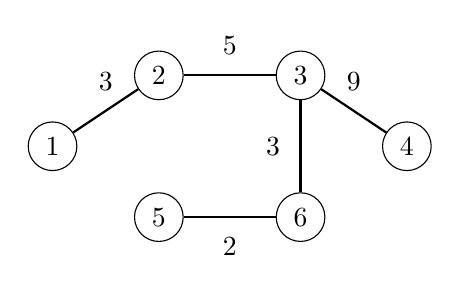
\begin{tikzpicture}[scale=0.9]
\node[draw, circle] (1) at (1.5,2) {$1$};
\node[draw, circle] (2) at (3,3) {$2$};
\node[draw, circle] (3) at (5,3) {$3$};
\node[draw, circle] (4) at (6.5,2) {$4$};
\node[draw, circle] (5) at (3,1) {$5$};
\node[draw, circle] (6) at (5,1) {$6$};
\path[draw,thick,-] (1) -- node[font=\small,label=above:3] {} (2);
\path[draw,thick,-] (2) -- node[font=\small,label=above:5] {} (3);
\path[draw,thick,-] (3) -- node[font=\small,label=above:9] {} (4);
\path[draw,thick,-] (5) -- node[font=\small,label=below:2] {} (6);
\path[draw,thick,-] (3) -- node[font=\small,label=left:3] {} (6);
\end{tikzpicture}
\end{center}

\index{minimum spanning tree}

全域木の重さとはエッジの重みの合計です。
上の全域木の重みは、$3+5+9+3+2 = 22$です。
\key{最小全域木(minimum spanning tree)}は、全ての全域木の中で最も重さが小さな全域木です。
先ほどの例では、次の最小全域木は重さが20です。

\begin{center}
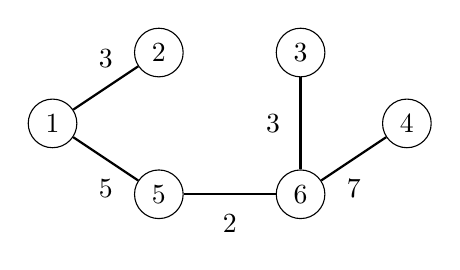
\begin{tikzpicture}[scale=0.9]
\node[draw, circle] (1) at (1.5,2) {$1$};
\node[draw, circle] (2) at (3,3) {$2$};
\node[draw, circle] (3) at (5,3) {$3$};
\node[draw, circle] (4) at (6.5,2) {$4$};
\node[draw, circle] (5) at (3,1) {$5$};
\node[draw, circle] (6) at (5,1) {$6$};

\path[draw,thick,-] (1) -- node[font=\small,label=above:3] {} (2);
\path[draw,thick,-] (1) -- node[font=\small,label=below:5] {} (5);
\path[draw,thick,-] (5) -- node[font=\small,label=below:2] {} (6);
\path[draw,thick,-] (6) -- node[font=\small,label=below:7] {} (4);
\path[draw,thick,-] (3) -- node[font=\small,label=left:3] {} (6);
\end{tikzpicture}
\end{center}

\index{maximum spanning tree}

\key{最大全域木(maximum spanning tree)}
は重さが最大となる木です。先の例では次のように重さ32の最大全域木ができます。

\begin{center}
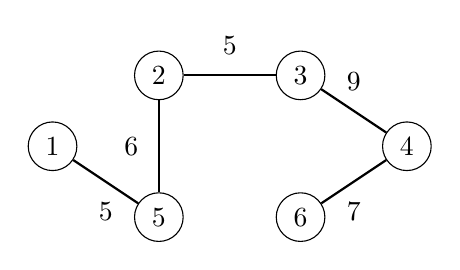
\begin{tikzpicture}[scale=0.9]
\node[draw, circle] (1) at (1.5,2) {$1$};
\node[draw, circle] (2) at (3,3) {$2$};
\node[draw, circle] (3) at (5,3) {$3$};
\node[draw, circle] (4) at (6.5,2) {$4$};
\node[draw, circle] (5) at (3,1) {$5$};
\node[draw, circle] (6) at (5,1) {$6$};
\path[draw,thick,-] (2) -- node[font=\small,label=above:5] {} (3);
\path[draw,thick,-] (3) -- node[font=\small,label=above:9] {} (4);
\path[draw,thick,-] (1) -- node[font=\small,label=below:5] {} (5);
\path[draw,thick,-] (6) -- node[font=\small,label=below:7] {} (4);
\path[draw,thick,-] (2) -- node[font=\small,label=left:6] {} (5);
\end{tikzpicture}
\end{center}

ここで、最小全域木・最大全域木になるグラフ(木)は複数存在することがあります。
これらの全域木は貪欲な方法で求めることができます。この章では、2つのアルゴリズムについて説明します。
説明では最小全域木のみに絞って説明を行いますが、最大全域木の場合は処理する辺の順を逆とすれば良いです。

\section{クラスカル法 - Kruskal's algorithm}

\index{Kruskal's algorithm}

\key{Kruskal法}
\footnote{このアルゴリズムは1956年にJ. B. Kruskalによって発表された \cite{kru56}.}
は次のように動作します。
まず、辺がなくノードだけのグラフを考えます。次に、このアルゴリズムは重みが小さい順に辺を調べて
サイクルを作らない場合は常にグラフにエッジを追加します。
このアルゴリズムは木を連結成分を保持してながら行います。
初期状態は各ノードは別々の連結成分に属しており、
木にエッジを追加する時にその2つの成分を結合します。
最終的にすべてのノードは同じ成分に属し、最小全域木となります。

\subsubsection{例}

\begin{samepage}
次のグラフを考えます。
\begin{center}
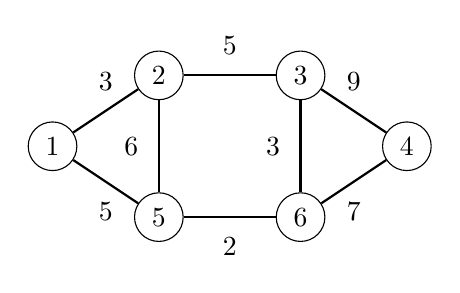
\begin{tikzpicture}[scale=0.9]
\node[draw, circle] (1) at (1.5,2) {$1$};
\node[draw, circle] (2) at (3,3) {$2$};
\node[draw, circle] (3) at (5,3) {$3$};
\node[draw, circle] (4) at (6.5,2) {$4$};
\node[draw, circle] (5) at (3,1) {$5$};
\node[draw, circle] (6) at (5,1) {$6$};
\path[draw,thick,-] (1) -- node[font=\small,label=above:3] {} (2);
\path[draw,thick,-] (2) -- node[font=\small,label=above:5] {} (3);
\path[draw,thick,-] (3) -- node[font=\small,label=above:9] {} (4);
\path[draw,thick,-] (1) -- node[font=\small,label=below:5] {} (5);
\path[draw,thick,-] (5) -- node[font=\small,label=below:2] {} (6);
\path[draw,thick,-] (6) -- node[font=\small,label=below:7] {} (4);
\path[draw,thick,-] (2) -- node[font=\small,label=left:6] {} (5);
\path[draw,thick,-] (3) -- node[font=\small,label=left:3] {} (6);
\end{tikzpicture}
\end{center}
\end{samepage}

\begin{samepage}
最初に全てのエッジを重みが小さい順にソートします。

\begin{tabular}{ll}
\\
edge & weight \\
\hline
5--6 & 2 \\
1--2 & 3 \\
3--6 & 3 \\
1--5 & 5 \\
2--3 & 5 \\
2--5 & 6 \\
4--6 & 7 \\
3--4 & 9 \\
\\
\end{tabular}
\end{samepage}

リストを上から処理し、各辺が2つの別の連結成分を結合するなら、その辺を接続します。

\begin{center}
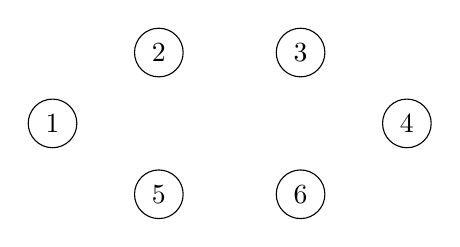
\begin{tikzpicture}[scale=0.9]
\node[draw, circle] (1) at (1.5,2) {$1$};
\node[draw, circle] (2) at (3,3) {$2$};
\node[draw, circle] (3) at (5,3) {$3$};
\node[draw, circle] (4) at (6.5,2) {$4$};
\node[draw, circle] (5) at (3,1) {$5$};
\node[draw, circle] (6) at (5,1) {$6$};
%\path[draw,thick,-] (1) -- node[font=\small,label=above:3] {} (2);
%\path[draw,thick,-] (2) -- node[font=\small,label=above:5] {} (3);
%\path[draw,thick,-] (3) -- node[font=\small,label=above:9] {} (4);
%\path[draw,thick,-] (1) -- node[font=\small,label=below:5] {} (5);
%\path[draw,thick,-] (5) -- node[font=\small,label=below:2] {} (6);
%\path[draw,thick,-] (6) -- node[font=\small,label=below:7] {} (4);
%\path[draw,thick,-] (2) -- node[font=\small,label=left:6] {} (5);
%\path[draw,thick,-] (3) -- node[font=\small,label=left:3] {} (6);
\end{tikzpicture}
\end{center}
まず、5--6 の処理は$\{5\}$ と $\{6\}$を連結し、
$\{5,6\}$とします。

\begin{center}
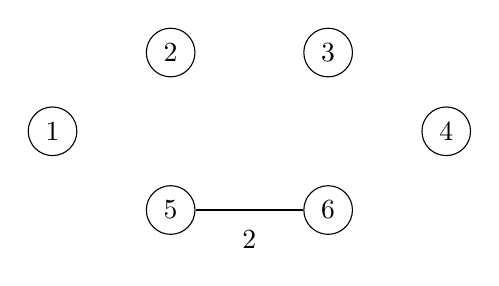
\begin{tikzpicture}
\node[draw, circle] (1) at (1.5,2) {$1$};
\node[draw, circle] (2) at (3,3) {$2$};
\node[draw, circle] (3) at (5,3) {$3$};
\node[draw, circle] (4) at (6.5,2) {$4$};
\node[draw, circle] (5) at (3,1) {$5$};
\node[draw, circle] (6) at (5,1) {$6$};

%\path[draw,thick,-] (1) -- node[font=\small,label=above:3] {} (2);
%\path[draw,thick,-] (2) -- node[font=\small,label=above:5] {} (3);
%\path[draw,thick,-] (3) -- node[font=\small,label=above:9] {} (4);
%\path[draw,thick,-] (1) -- node[font=\small,label=below:5] {} (5);
\path[draw,thick,-] (5) -- node[font=\small,label=below:2] {} (6);
%\path[draw,thick,-] (6) -- node[font=\small,label=below:7] {} (4);
%\path[draw,thick,-] (2) -- node[font=\small,label=left:6] {} (5);
%\path[draw,thick,-] (3) -- node[font=\small,label=left:3] {} (6);
\end{tikzpicture}
\end{center}
同じように、 1--2, 3--6, 1--5 が接続されます。

\begin{center}
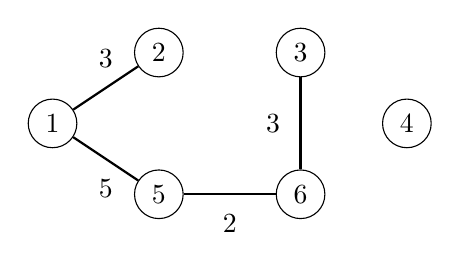
\begin{tikzpicture}[scale=0.9]
\node[draw, circle] (1) at (1.5,2) {$1$};
\node[draw, circle] (2) at (3,3) {$2$};
\node[draw, circle] (3) at (5,3) {$3$};
\node[draw, circle] (4) at (6.5,2) {$4$};
\node[draw, circle] (5) at (3,1) {$5$};
\node[draw, circle] (6) at (5,1) {$6$};

\path[draw,thick,-] (1) -- node[font=\small,label=above:3] {} (2);
%\path[draw,thick,-] (2) -- node[font=\small,label=above:5] {} (3);
%\path[draw,thick,-] (3) -- node[font=\small,label=above:9] {} (4);
\path[draw,thick,-] (1) -- node[font=\small,label=below:5] {} (5);
\path[draw,thick,-] (5) -- node[font=\small,label=below:2] {} (6);
%\path[draw,thick,-] (6) -- node[font=\small,label=below:7] {} (4);
%\path[draw,thick,-] (2) -- node[font=\small,label=left:6] {} (5);
\path[draw,thick,-] (3) -- node[font=\small,label=left:3] {} (6);
\end{tikzpicture}
\end{center}

これらのステップの後、ほとんどの連結成分は結合され、2つの連結成分が存在します。
$\{1,2,3,5,6\}$と$\{4\}$です。

次に処理するのは2--3ですが、同じ連結成分に含まれるので接続しません。 2--5も同様です。

\begin{samepage}
最後に、4--6が接続されます。

\begin{center}
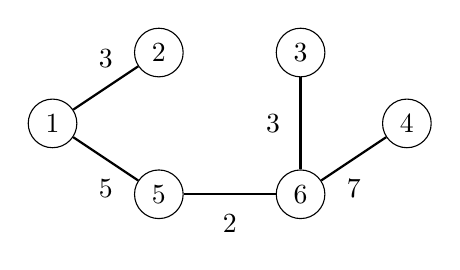
\begin{tikzpicture}[scale=0.9]
\node[draw, circle] (1) at (1.5,2) {$1$};
\node[draw, circle] (2) at (3,3) {$2$};
\node[draw, circle] (3) at (5,3) {$3$};
\node[draw, circle] (4) at (6.5,2) {$4$};
\node[draw, circle] (5) at (3,1) {$5$};
\node[draw, circle] (6) at (5,1) {$6$};

\path[draw,thick,-] (1) -- node[font=\small,label=above:3] {} (2);
%\path[draw,thick,-] (2) -- node[font=\small,label=above:5] {} (3);
%\path[draw,thick,-] (3) -- node[font=\small,label=above:9] {} (4);
\path[draw,thick,-] (1) -- node[font=\small,label=below:5] {} (5);
\path[draw,thick,-] (5) -- node[font=\small,label=below:2] {} (6);
\path[draw,thick,-] (6) -- node[font=\small,label=below:7] {} (4);
%\path[draw,thick,-] (2) -- node[font=\small,label=left:6] {} (5);
\path[draw,thick,-] (3) -- node[font=\small,label=left:3] {} (6);
\end{tikzpicture}
\end{center}
\end{samepage}

これで全ての点が同じ連結成分に含まれるので処理を終えます。
重さが$2+3+3+5+7=20$の最小全域木ができました。

\subsubsection{なぜこれで良いか?}

これでなぜ最小全域木が求められるのでしょう?
最小の重みの辺が含まれないことを考えます。
例えば、先ほどの例で最小重みの辺5--6 が含まれないとします。
そのようなグラフは複数考えられますが、例えば次のような木を考えましょう。

\begin{center}
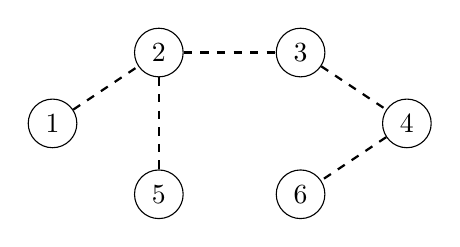
\begin{tikzpicture}[scale=0.9]
\node[draw, circle] (1) at (1.5,2) {$1$};
\node[draw, circle] (2) at (3,3) {$2$};
\node[draw, circle] (3) at (5,3) {$3$};
\node[draw, circle] (4) at (6.5,2) {$4$};
\node[draw, circle] (5) at (3,1) {$5$};
\node[draw, circle] (6) at (5,1) {$6$};

\path[draw,thick,-,dashed] (1) -- (2);
\path[draw,thick,-,dashed] (2) -- (5);
\path[draw,thick,-,dashed] (2) -- (3);
\path[draw,thick,-,dashed] (3) -- (4);
\path[draw,thick,-,dashed] (4) -- (6);
\end{tikzpicture}
\end{center}


しかし、この木が最小全域木ではありません。
木からある辺を取り除き、5--6に置き換えることができ、さらに重さの小さな木ができます。

\begin{center}
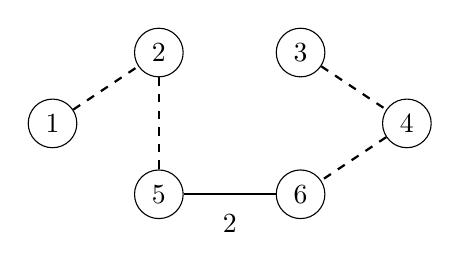
\begin{tikzpicture}[scale=0.9]
\node[draw, circle] (1) at (1.5,2) {$1$};
\node[draw, circle] (2) at (3,3) {$2$};
\node[draw, circle] (3) at (5,3) {$3$};
\node[draw, circle] (4) at (6.5,2) {$4$};
\node[draw, circle] (5) at (3,1) {$5$};
\node[draw, circle] (6) at (5,1) {$6$};

\path[draw,thick,-,dashed] (1) -- (2);
\path[draw,thick,-,dashed] (2) -- (5);
\path[draw,thick,-,dashed] (3) -- (4);
\path[draw,thick,-,dashed] (4) -- (6);
\path[draw,thick,-] (5) -- node[font=\small,label=below:2] {} (6);
\end{tikzpicture}
\end{center}

このため、最小の重さの辺を最小全域木に含めることは妥当で最小のスパニングツリーが生成されます。
重さが小さな順に辺を木に加えることが最適であることを示すことができ、
クラスカルのアルゴリズムは正しく動作して常に最小全域木となることが示されました。

\subsubsection{実装}

クラスカル法の実装は辺をリスト表現で持つのが便利です。
最初に$O(m log m)$でリスト中のエッジを重さ順にソートし、
次に以下のように最小スパニングツリーを構築します。

\begin{lstlisting}
for (...) {
  if (!same(a,b)) unite(a,b);
}
\end{lstlisting}

ループは$a,b$を処理します。$same$は同じ連結成分にいるかを判定する関数で、
$unite$は互いに所属する連結成分を結合する操作です。これらをシンプルに書くと
$O(log(n+m))$となってしまいますが$Union-Find$を用いるとこれらは$O(log n)$で実装することができるため、
ソート後の計算量$O(m log n)$を実現できます。

\section{Union-find構造 - Union-find structure}

\index{union-find structure}

\key{Union-find構造} は集合の集まりを管理するデータ構造です。
どの要素もいずれかの集合に属し、2つ以上の集合に属しません。
この構造は先にあげた$unite$と$same$を$O(\log n)$で実行できます。
\footnote{ ここで紹介する構造は、1971年にJ. D. HopcroftとJ. D. Ullmanによって紹介されたもの \cite{hop71}。
その後、1975年にR. E. Tarjanがこの構造のより洗練された変種を研究し\cite{tar75}、
現在では 多くのアルゴリズムの教科書で議論されています。}

\subsubsection{構造}

Union-findでは各集合の1つの要素がその集合の代表として存在します。
そして、集合の他の要素は必ず代表への連鎖に辿ることができます。

集合が$\{1, 4, 7\}$、\{5\}、\{2, 3, 6, 8\}としましょう。
\begin{center}
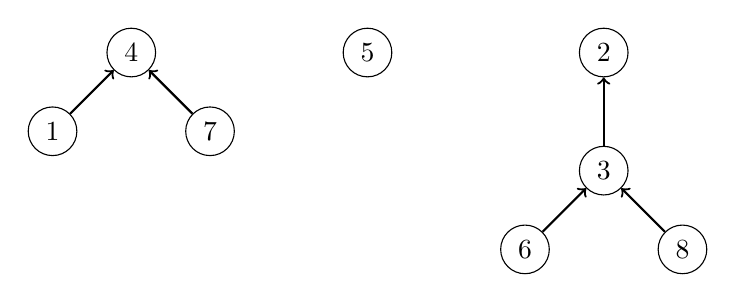
\begin{tikzpicture}
\node[draw, circle] (1) at (0,-1) {$1$};
\node[draw, circle] (2) at (7,0) {$2$};
\node[draw, circle] (3) at (7,-1.5) {$3$};
\node[draw, circle] (4) at (1,0) {$4$};
\node[draw, circle] (5) at (4,0) {$5$};
\node[draw, circle] (6) at (6,-2.5) {$6$};
\node[draw, circle] (7) at (2,-1) {$7$};
\node[draw, circle] (8) at (8,-2.5) {$8$};

\path[draw,thick,->] (1) -- (4);
\path[draw,thick,->] (7) -- (4);

\path[draw,thick,->] (3) -- (2);
\path[draw,thick,->] (6) -- (3);
\path[draw,thick,->] (8) -- (3);

\end{tikzpicture}
\end{center}
この図では集合の代表は4、5、2です。
あるの要素の代表は、その要素から木を辿ると発見できます。
例えば、 $6 \rightarrow 3 \rightarrow 2$という連鎖をたどれば、要素2が要素6の代表です。
2つの要素が同じ集合に属するのは、その代表が同じであるときだけです。
2つの集合は、一方の集合の代表と他方の集合の代表を結ぶことで結合することができます。
例えば、$\{1,4,7\}$ と $\{2,3,6,8\}$は以下のように結合することができます。

\begin{center}
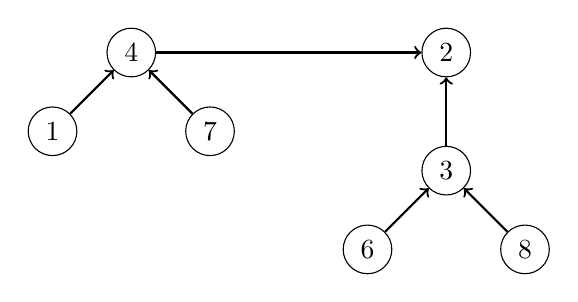
\begin{tikzpicture}
\node[draw, circle] (1) at (2,-1) {$1$};
\node[draw, circle] (2) at (7,0) {$2$};
\node[draw, circle] (3) at (7,-1.5) {$3$};
\node[draw, circle] (4) at (3,0) {$4$};
\node[draw, circle] (6) at (6,-2.5) {$6$};
\node[draw, circle] (7) at (4,-1) {$7$};
\node[draw, circle] (8) at (8,-2.5) {$8$};

\path[draw,thick,->] (1) -- (4);
\path[draw,thick,->] (7) -- (4);

\path[draw,thick,->] (3) -- (2);
\path[draw,thick,->] (6) -- (3);
\path[draw,thick,->] (8) -- (3);

\path[draw,thick,->] (4) -- (2);
\end{tikzpicture}
\end{center}

結果、$\{1,2,3,4,6,7,8\}$の要素が集合に含まれ、要素2がそれらの集合全体の代表となり、
もともと代表要素4であった要素2を指すようになります。
Union-findの操作の計算量は集合をどのように結合するかに依存します。
良い工夫は小さい集合を大きい集合の代表要素に繋ぎます(同じ大きさの集合の場合どちらを大きい方とみなしてもよいです)。
この方法を用いるとどのパスの長さも$O( \log n)$となるので、
対応する辺を辿る中で任意の要素の代表を効率的に求めることができます。

\subsubsection{実装 - Implementation}

union-findは、
配列を使用して実装できます。
以下の実装では ,配列 \texttt{link} は各要素について,
親となる要素(代表であればその要素自身)を含み,
配列 \texttt{size} は
各代表について,対応する集合の大きさを保持します。

初期状態では、各要素は別々の集合に属しています。
\begin{lstlisting}
for (int i = 1; i <= n; i++) link[i] = i;
for (int i = 1; i <= n; i++) size[i] = 1;
\end{lstlisting}

関数\texttt{find}は,
ある要素$x$の代表を返します。
代表は$x$から始まる鎖をたどって見つけることができます。

\begin{lstlisting}
int find(int x) {
    while (x != link[x]) x = link[x];
    return x;
}
\end{lstlisting}

関数\texttt{same} は要素$a$,$b$が同じ集合に属するかどうかをチェックする関数で、
関数\texttt{find}を使うことで簡単に実現できます。

\begin{lstlisting}
bool same(int a, int b) {
    return find(a) == find(b);
}
\end{lstlisting}

\begin{samepage}
関数 \texttt{unite}  は,
要素 $a$ と $b$ を含む集合を結合する関数です。
この時、要素は異なる集合に存 在しなければなりません。
この関数は,まず集合の代表を求め,
次に小さい方の集合を大きい方の集合に接続します.

\begin{lstlisting}
void unite(int a, int b) {
    a = find(a);
    b = find(b);
    if (size[a] < size[b]) swap(a,b);
    size[a] += size[b];
    link[b] = a;
}
\end{lstlisting}
\end{samepage}

関数\texttt{find}の時間計算量は、
各鎖の長さが$O(\log n)$ であると仮定すると、
$O(\log n)$ で動作します。
この場合、関数\texttt{same} と \texttt{unite}も
$O(\log n)$ の時間で動作します。
関数 \texttt{unite} は、
小さい集合を大きい集合に接続することで
、各木の長さが最長で $O(\log n)$ であることを保証できます。

\section{プリムのアルゴリズム - Prim's algorithm}

\index{プリムのアルゴリズム - Prim's algorithm}

\key{プリムのアルゴリズム - Prim's algorithm}\footnote{The algorithm is
named after R. C. Prim who published it in 1957 \cite{pri57}.
However, the same algorithm was discovered already in 1930
by V. Jarník.} 
は最小全域木を求めるための手法です。
このアルゴリズムでは、
まず各ノードを独立した木に追加します。
その後は常に最小コストの辺を選択して新しいノードを木に追加します。
最後に、すべてのノードが一つの木に追加され最小全域木が発見されます。

プリムのアルゴリズムはダイクストラのアルゴリズムに似ています。
ダイクストラのアルゴリズムは常に開始ノードからの距離が最小となるエッジを選択しますが、
プリムのアルゴリズムは単に新しいノードを木に追加する最小コストの辺を選んでいきます。

\subsubsection{例 - Example}

動作を図で見ていきましょう。

\begin{center}
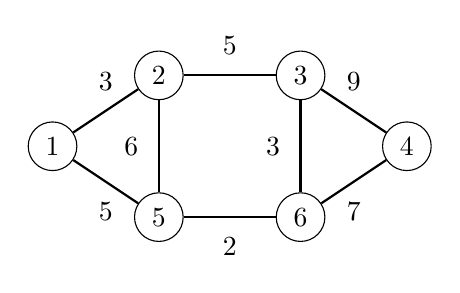
\begin{tikzpicture}[scale=0.9]
\node[draw, circle] (1) at (1.5,2) {$1$};
\node[draw, circle] (2) at (3,3) {$2$};
\node[draw, circle] (3) at (5,3) {$3$};
\node[draw, circle] (4) at (6.5,2) {$4$};
\node[draw, circle] (5) at (3,1) {$5$};
\node[draw, circle] (6) at (5,1) {$6$};
\path[draw,thick,-] (1) -- node[font=\small,label=above:3] {} (2);
\path[draw,thick,-] (2) -- node[font=\small,label=above:5] {} (3);
\path[draw,thick,-] (3) -- node[font=\small,label=above:9] {} (4);
\path[draw,thick,-] (1) -- node[font=\small,label=below:5] {} (5);
\path[draw,thick,-] (5) -- node[font=\small,label=below:2] {} (6);
\path[draw,thick,-] (6) -- node[font=\small,label=below:7] {} (4);
\path[draw,thick,-] (2) -- node[font=\small,label=left:6] {} (5);
\path[draw,thick,-] (3) -- node[font=\small,label=left:3] {} (6);

%\path[draw=red,thick,-,line width=2pt] (5) -- (6);
\end{tikzpicture}
\end{center}
最初は全てのノードは独立しています。
\begin{center}
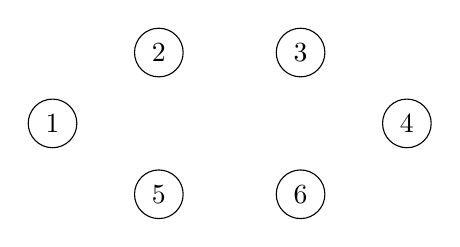
\begin{tikzpicture}[scale=0.9]
\node[draw, circle] (1) at (1.5,2) {$1$};
\node[draw, circle] (2) at (3,3) {$2$};
\node[draw, circle] (3) at (5,3) {$3$};
\node[draw, circle] (4) at (6.5,2) {$4$};
\node[draw, circle] (5) at (3,1) {$5$};
\node[draw, circle] (6) at (5,1) {$6$};
%\path[draw,thick,-] (1) -- node[font=\small,label=above:3] {} (2);
%\path[draw,thick,-] (2) -- node[font=\small,label=above:5] {} (3);
%\path[draw,thick,-] (3) -- node[font=\small,label=above:9] {} (4);
%\path[draw,thick,-] (1) -- node[font=\small,label=below:5] {} (5);
%\path[draw,thick,-] (5) -- node[font=\small,label=below:2] {} (6);
%\path[draw,thick,-] (6) -- node[font=\small,label=below:7] {} (4);
%\path[draw,thick,-] (2) -- node[font=\small,label=left:6] {} (5);
%\path[draw,thick,-] (3) -- node[font=\small,label=left:3] {} (6);
\end{tikzpicture}
\end{center}
任意のノードを開始ノードとしてよいのでノード1を選択したとします。
まず、重み3のエッジで結ばれているノード2を追加しましょう。
\begin{center}
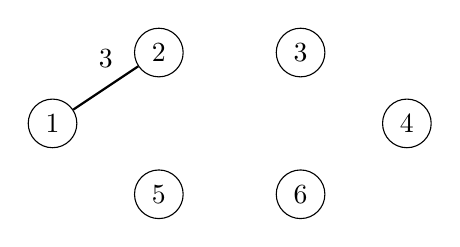
\begin{tikzpicture}[scale=0.9]
\node[draw, circle] (1) at (1.5,2) {$1$};
\node[draw, circle] (2) at (3,3) {$2$};
\node[draw, circle] (3) at (5,3) {$3$};
\node[draw, circle] (4) at (6.5,2) {$4$};
\node[draw, circle] (5) at (3,1) {$5$};
\node[draw, circle] (6) at (5,1) {$6$};
\path[draw,thick,-] (1) -- node[font=\small,label=above:3] {} (2);
%\path[draw,thick,-] (2) -- node[font=\small,label=above:5] {} (3);
%\path[draw,thick,-] (3) -- node[font=\small,label=above:9] {} (4);
%\path[draw,thick,-] (1) -- node[font=\small,label=below:5] {} (5);
%\path[draw,thick,-] (5) -- node[font=\small,label=below:2] {} (6);
%\path[draw,thick,-] (6) -- node[font=\small,label=below:7] {} (4);
%\path[draw,thick,-] (2) -- node[font=\small,label=left:6] {} (5);
%\path[draw,thick,-] (3) -- node[font=\small,label=left:3] {} (6);
\end{tikzpicture}
\end{center}

この後、重み5を持つ辺は2本あるので、
ノード3かノード5のどちらかを木に追加できます。
ノード3を追加します。

\begin{center}
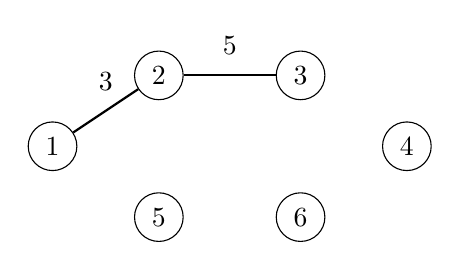
\begin{tikzpicture}[scale=0.9]
\node[draw, circle] (1) at (1.5,2) {$1$};
\node[draw, circle] (2) at (3,3) {$2$};
\node[draw, circle] (3) at (5,3) {$3$};
\node[draw, circle] (4) at (6.5,2) {$4$};
\node[draw, circle] (5) at (3,1) {$5$};
\node[draw, circle] (6) at (5,1) {$6$};
\path[draw,thick,-] (1) -- node[font=\small,label=above:3] {} (2);
\path[draw,thick,-] (2) -- node[font=\small,label=above:5] {} (3);
%\path[draw,thick,-] (3) -- node[font=\small,label=above:9] {} (4);
%\path[draw,thick,-] (1) -- node[font=\small,label=below:5] {} (5);
%\path[draw,thick,-] (5) -- node[font=\small,label=below:2] {} (6);
%\path[draw,thick,-] (6) -- node[font=\small,label=below:7] {} (4);
%\path[draw,thick,-] (2) -- node[font=\small,label=left:6] {} (5);
%\path[draw,thick,-] (3) -- node[font=\small,label=left:3] {} (6);
\end{tikzpicture}
\end{center}

\begin{samepage}
これを繰り返します。
\begin{center}
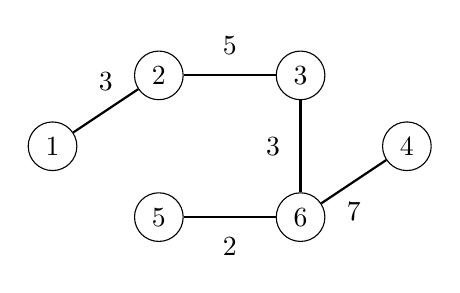
\begin{tikzpicture}[scale=0.9]
\node[draw, circle] (1) at (1.5,2) {$1$};
\node[draw, circle] (2) at (3,3) {$2$};
\node[draw, circle] (3) at (5,3) {$3$};
\node[draw, circle] (4) at (6.5,2) {$4$};
\node[draw, circle] (5) at (3,1) {$5$};
\node[draw, circle] (6) at (5,1) {$6$};
\path[draw,thick,-] (1) -- node[font=\small,label=above:3] {} (2);
\path[draw,thick,-] (2) -- node[font=\small,label=above:5] {} (3);
%\path[draw,thick,-] (3) -- node[font=\small,label=above:9] {} (4);
%\path[draw,thick,-] (1) -- node[font=\small,label=below:5] {} (5);
\path[draw,thick,-] (5) -- node[font=\small,label=below:2] {} (6);
\path[draw,thick,-] (6) -- node[font=\small,label=below:7] {} (4);
%\path[draw,thick,-] (2) -- node[font=\small,label=left:6] {} (5);
\path[draw,thick,-] (3) -- node[font=\small,label=left:3] {} (6);
\end{tikzpicture}
\end{center}
\end{samepage}

\subsubsection{実装 - Implementation}

ダイクストラのアルゴリズムと同様に、
プリムのアルゴリズムも優先度付きキューを用いて効率的に実装できます。
優先度付きキューには、1本のエッジを使って現在のコンポーネントに接続できるすべてのノードと
そのエッジの重みの昇順に格納しておきます。

プリムのアルゴリズムの時間計算量は$O(n + m \log m)$で、
ダイクストラのアルゴリズムの時間計算量と同じです。
実際には、プリムのアルゴリズムとクラシカルのアルゴリズムはどちらも効率的で、
アルゴリズムの選択は好みの問題です。
ただし、クラシカル法が用いられることが多いです。